\begin{frame}{Services (Applikation)}
	\begin{itemize}
		\item Embedded System besteht meist aus mehreren Prozessen $\rightarrow$ Microservices
		\item Webserver, Prozessueberwachung, SSH, FTP, UI
		\item standard linux tools (busybox)
		\item libraries
		\item packetmanager
		\item Hardware Ansteuerung
		\item gutes IPC system (z.B. kdbus)
		\item eigener Service
		\begin{itemize}
			\item reaktiv, event-getriggert
			\item Qt gut geeignet
		\end{itemize}
	\end{itemize}
\end{frame}

\begin{frame}{Hardware ansteuern}
	\begin{multicols}{2}
		\begin{center}
			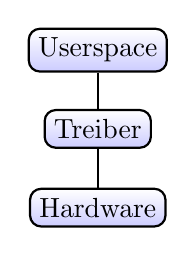
\begin{tikzpicture}[thick,
				every node/.style = {shape=rectangle, rounded corners,
					draw, align=center,
					top color=white, bottom color=blue!20}]]

				\node (userspace) {Userspace};
				\node[below of=userspace] (driver) {Treiber};
				\node[below of=driver] (hardware) {Hardware};
				
				\draw (userspace) to (driver);
				\draw (driver) to (hardware);
			\end{tikzpicture}
			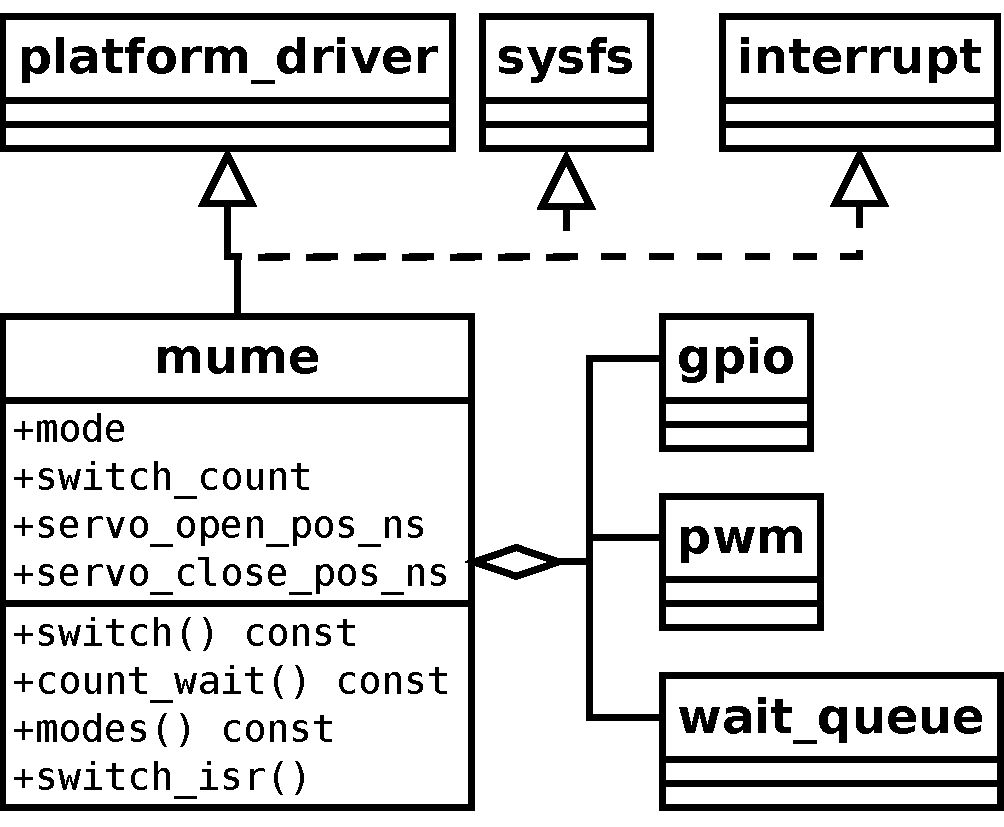
\includegraphics[width=0.5\textwidth]{res/mumedriver}
		\end{center}
	\end{multicols}
	\begin{itemize}
		\item wie können wir die Hardware ansteuern?
		\item[$\rightarrow$] Linux Treiber, Frameworks, Infrastructure:
		\begin{itemize}
			\item Framework für Treiber
			\item Infrastrukur um auf Subsysteme zuzugreifen
		\end{itemize}
	\end{itemize}
\end{frame}

\begin{frame}{MUME Service}
	\begin{itemize}
		\item wie können wir den Treiber ansprechen?
		\item[$\rightarrow$] sysfs
		\item mumesrv als Userspace-Teil des Treibers:
		\begin{itemize}
			\item Zugriff via D-Bus
			\item ablegen persistenter Daten (counter, open/close position)
			\item Kommunikation mit Treiber
		\end{itemize}
	\end{itemize}
\end{frame}

\begin{frame}{GUI}
	\begin{itemize}
		\item Browser Zugriff auf System?
		\item[$\rightarrow$] Web-Service
		\begin{itemize}
			\item nginx
			\item fastcgi
			\item mumeweb
			\begin{itemize}
				\item Kommunikation via D-Bus mit mumesrv
			\end{itemize}
		\end{itemize}
	\end{itemize}
\end{frame}

\begin{frame}{Service Manager}
	\begin{itemize}
		\item Wie starten und managen wir die Services?
		\item[$\rightarrow$] systemd
		\begin{itemize}
			\item service files schreiben
		\end{itemize}
	\end{itemize}
\end{frame}

\begin{frame}{Produktiv Image}
	\begin{itemize}
		\item Wie können wir die Firmware verteilen?
		\item[$\rightarrow$] Yocto
		\begin{itemize}
			\item Rezepte für Services
			\item anpassen bestehender Rezepte (nginx, qt, \ldots)
			\item Rezept für image
		\end{itemize}
		\item bitbake image
	\end{itemize}
\end{frame}

\begin{frame}{Was passiert bei einem Tastendruck in der Web-Applikation}
	Geht runter:
	\begin{itemize}
		\item SVG, Javascript
		\item XML/HTTP
		\item FastCGI
		\item MumeWeb
		\item D-Bus
		\item MumeSrv
		\item SysFS
		\item Kernel
		\item MUME-Treiber
		\item PWM
		\item Servo bewegt sich!
	\end{itemize}
\end{frame}

\begin{frame}{Echtzeit}
	\begin{itemize}
		\item Bearbeitung ist nach einer bestimmten Zeit nach dem auftreten eines Ereignisses abgeschlossen.
		\item Die Bearbeitung eines Interrupts dauert nie laenger als $t$.
		\item bei weicher Echtzeit ist dieses Verhalten wuenschenswert (Video wiedergabe)
		\item jeder Treiber kann Interrupts sperren
		\item Swapping
		\item Prozessoren mit Caches haben undefinierbares Verhalten, abschalten nicht Sinn der Sache
		\item Loesung ist separater uC, im selben oder eigenen DIE
	\end{itemize}
\end{frame}
